\section{Ensemble strategies}
\label{sec:ensembles}

Inconsistency between explanations of different ML models poses a significant challenge, where choices as arbitrary as the random seed used during the training phase of a deployed ML model can drastically affect the explanation provided to a particular individual \citep{brunet2022, damour2022}. Ensembling provides a promising avenue for aligning the explanations across similarly performing models. However, conventional or \textit{vanilla} methods may necessitate a prohibitively large number of models to do so.

Given this context, the primary question driving our research is:

\begin{quote}
\centering
\textit{Can we maximize (in expectation) the explanation similarity between two ensembles constructed from $n$ samples of the underspecification set?} 
\end{quote}
%\suraj{Should we define "underspecification set" concretely before this?}

This question underscores our exploration of ensemble methods towards bridging the gap between computational efficiency and explanation consistency. Once a sufficiently large underspecification set has been formed for a given dataset and task, samples of equally performing models are used to construct ensembles. We proceed to outline our ensembling strategies (summarized in Figure~\ref{fig:weight_space}).

% \subsection{Vanilla ensembles (work in progress)}
% \label{subsec:ensembles_vanilla}

% In our setup we consider as baselines two traditional forms of ensembles: a) the \textit{average} output of all constituent models, and b) the \textit{majority vote} prediction. Specifically, for trained weights $\omega_i$, and corresponding model $f_{\omega_i}$, the average output of an $n$-sized ensemble on input $x$ is $\Bar{f}(x) = \frac{1}{n} \sum_{i} f_{\omega_i}(x)$, and the majority vote prediction is $\textit{mode}(F(x))$, where $F(x) = \{  {\mathrm{argmax}} \, f_{\omega_1}(x), {\mathrm{argmax}} \, f_{\omega_2}(x), \dots, {\mathrm{argmax}} \, f_{\omega_n}(x) \} $.

% \textit{Explanation of majority vote + notation.}

% \paragraph{Notation:} weights $\omega_i\in\mathcal{R}^W$, corresponding predictor $f_{\omega_i}$, soft prediction $f_{\omega_i}(x)$, hard prediction $\hat{f}_{\omega_i}(x) = \underset{y \in Y}{\mathrm{argmax}} \, f_{\omega_i}(x)_y$ ensemble function $E_F$, given a set of models $F = \{f_{\omega_1}, f_{\omega_2}, \ldots, f_{\omega_n}\}$.
% \suraj{I understand this is not done, but reminder to include dimensionalities of vectors, model outputs, etc.}

% The ensemble prediction for $x$ using the majority vote ensemble is $E_F(x) = \underset{y \in Y}{\mathrm{argmax}} \sum_{i=1}^{n} I(y = \hat{f}_{\omega_i}(x))$. Average: $E_F(x) = \frac{1}{n}\sum_{i=1}^n y_i(x)$

% We follow \cite{black2021selective}, average explanations across members that voted for the majority class.

% \paragraph{Explanations of ensembles}

% For explanation techniques satisfy distributivity --> average explanations --> treat as single model. True for gradients, smoothgrad, other gradient methods. Empirically true for DeepSHAP (confirm).

% For grad/sg, this property streamlines the generation and evaluation of ensemble explanations.

% \textit{Include DeepSHAP, confirm if distributivity holds (empirically it does).}

% \textit{What's the point? So we can make predictors that correspond to the explanations?}

% \paragraph{Defining ensemble size} In the context of our work, the \textit{size} of an ensemble refers to the number of pre-trained models used, and not the total number of models produced through later described techniques such as weight perturbation or mode connectivity. For instance, an ensemble that originates from a single pre-trained model, whose weights are then perturbed $n$ times, has an ensemble size of one under our definition. This is because no extra training is required to create the ensemble. We make this distinction to avoid confusion, and to accurately understand the computational efficiency of our methods. \textit{Alright, fix this carcrash of a paragraph. Gonna have to think on this one.}

\subsection{Ensembles via weight perturbation}
\label{subsec:ensembles_weight}

While we find that standard ensemble methods are capable of aligning the explanations of models from the underspecification set, they often require a large collection of pre-trained models to do so. To reduce the number of models needed for achieving explanation consistency, we propose a computationally cheap ensembling method that injects Gaussian noise $\epsilon \sim \mathcal{N}(0,\sigma^2)$ to the weights or biases of a given layer. Figure~\ref{fig:weight_space}, Center, depicts this in relation to the other methods.

\begin{figure}[t]
    \centering
    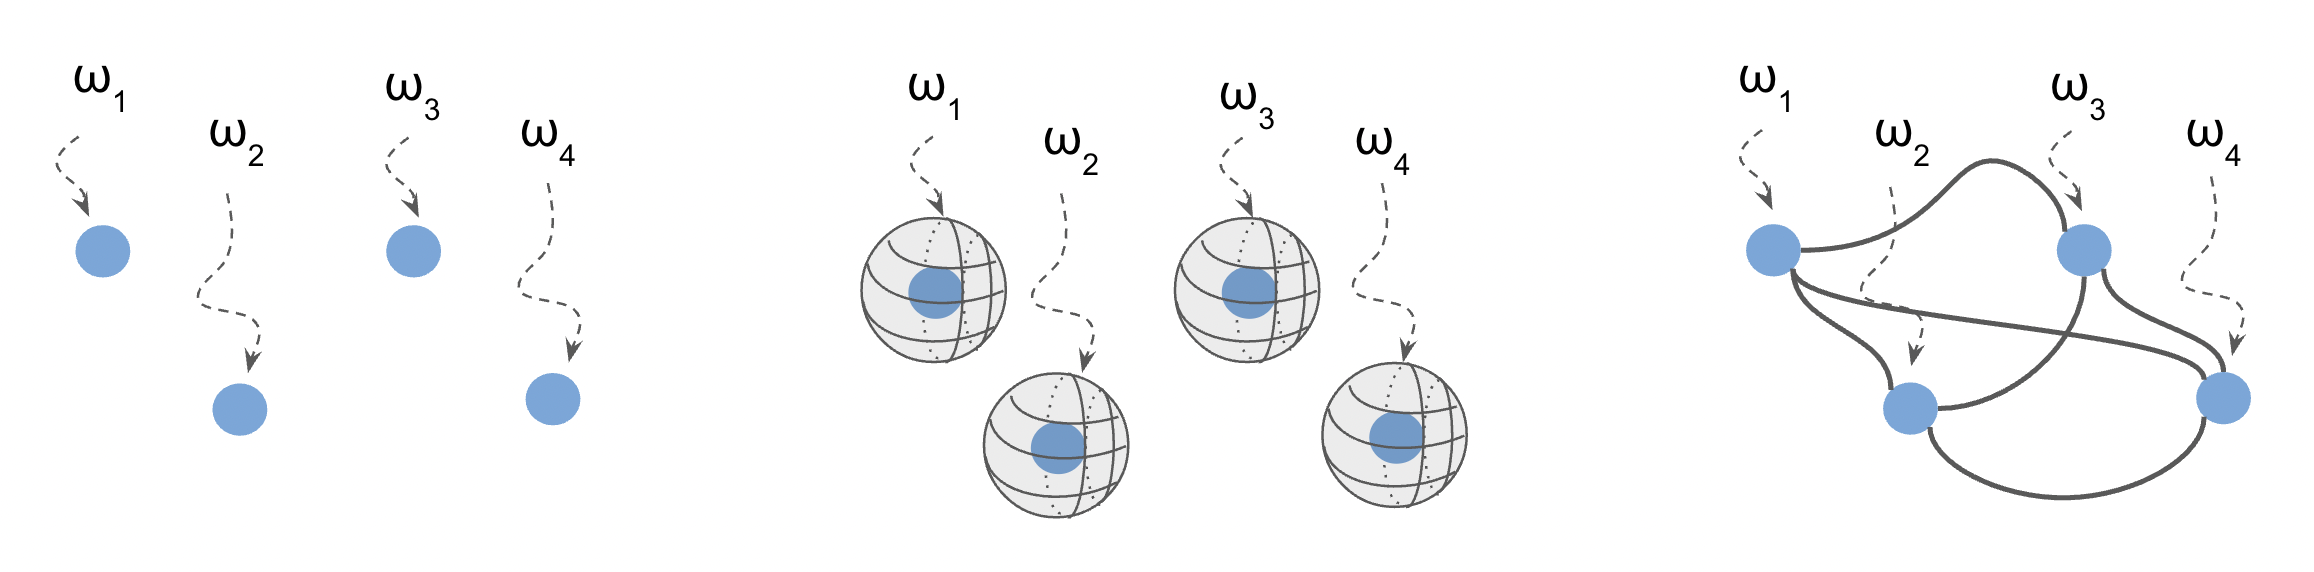
\includegraphics[width=0.9\textwidth]{figures/weight_space.png}
    \caption{\small Weight space visualizations of the methods we explore. \textbf{Left:} the underspecification set of (nearly) equally performing models, trained with the same hyperparameters but different random initializations. \textbf{Center:} local \textit{weight perturbations} to each of the models in the underspecification set, forming regions of alternate predictors of similar performance. The perturbations are themselves ensembled to form \textit{perturbed models}. \textbf{Right:} global \textit{mode connectivity} paths of near-constant loss, connecting different members of the underspecification set. Vanilla ensembling of models increases explanation consistency but requires an impractically large number of models. Our methods leverage ensembles formed by local weight perturbations and global mode-connected models to achieve better explanation consistency with fewer models and computational overhead.}
    \label{fig:weight_space}
\end{figure}

Constructing an ensemble using this method requires the weights of $n$ pre-trained models sampled from the underspecification set, each denoted $\omega_i$. The method perturbs each $\omega_i$ a total of $m$ times, leading to $m$ variants of each original model $f_{\omega_i}$. We denote the collection of the $m$ variants as the \textit{perturbed model} $f_{\Tilde{\omega}_i}$. This process of generating $n$ perturbed models does not involve the computational expense of training $n \times m$ distinct models from scratch. Instead, we capitalize on the learned knowledge of the $n$ pre-trained models, exploring the local regions surrounding their weights.
% Applying the linearity of model gradients, i.e. $\nabla_x \sum_i f_{\omega_i} = \sum_i \nabla_x f_{\omega_i}=\sum_i g_{\omega_i}$, for each perturbed model we have
% \[f_{\Tilde{\omega}_i}(x)=\frac{1}{m}\sum_{j=1}^m f_{\omega_i+\nu_j}(x) \ \ \Rightarrow \ \ \nabla f_{\Tilde{\omega}_i}=g_{\Tilde{\omega}_i}(x)=\frac{1}{m}\sum_{j=1}^m g_{\omega_i+\nu_j}(x)\]
 %The resulting ensemble is given as $E_{\Tilde{F}}(x)$, i.e. the ensemble of the $n$ perturbed models. \textit{This entire description requires clarification.}

Our approach draws inspiration from Smoothgrad \citep{smoothgrad2017}, which perturbs the input to stabilize the gradient estimation at a particular point. Unlike Smoothgrad, which provides an explanation for a smoothed approximation of a potentially noisy decision boundary, by perturbing the parameters directly and aggregating the results, this approach smooths both the explanation and the model's decision region. Techniques that perturb the parameters of ML models have been explored in prior work on adversarial training \citep{wu2020} and robust explanation generation \citep{upadhyay2021}, as well as more generally in the context of Bayesian learning \citep{gal2016, mackay1992}. Other conceptually similar examples to our approach are dropout \citep{srivastava2014}, and stochastic weight averaging \citep{izmailov2018}, a technique which promotes convergence of the SGD learning algorithm by averaging model weights during the final epochs of training. Informed by these works, we introduce weight perturbation as a computationally cheap ensembling strategy, with the specific goal of enhancing explanation similarity.


\subsection{Ensembles via mode connectivity}
\label{subsec:ensembles_mode}

Instead of sampling locally around a single model in weight space, we also consider global explorations between pairs of models along the constant paths of low loss found via mode connectivity \citep{garipov2018}. Quadratic Bezier curves provide a convenient parametrization of smooth paths, where the curve denoted $\phi_\theta(t)$ with endpoints $\omega_1$ and $\omega_2$ (sampled from the underspecification set) is given by 
\[\phi_\theta(t) = (1-t)^2 \omega_1 + 2t(1-t)\theta + t^2\omega_2, 0 \leq t \leq 1\]

Once such paths between pairs of models are obtained, ensembles can be constructed at little extra cost, most simply by uniformally sampling the scalar $t$, returning model weights along the path (Figure~\ref{fig:weight_space}, Right). To construct an ensemble from $n$ pre-trained models, we form connections between $n/2$ non-overlapping pairs, before sampling along these connections and ensembling the sampled weights. We discuss the curve finding procedure in \S\ref{sec:experiments}.


\subsection{Illustration on a toy example}
\label{subsec:ensembles_illustration}

In Figure~\ref{fig:toy_methods}, we illustrate the problem of explanatory multiplicity on the two moons dataset, and visualize the effectiveness of the described ensembling techniques in aligning the input gradients (saliency) of models. Observe that while vanilla ensembles (Left Center) constructed from four pre-trained models $f_{\omega_i}$ demonstrate reductions in average pairwise explanation difference compared to single models (Left), ensembles constructed from four perturbed models $f_{\Tilde{\omega}_i}$ effectively smooth the explanation distribution, achieving significantly better alignment (Right Center). We note similar smoothing effects for ensembles constructed via mode connectivity (Right), again using four pre-trained models i.e. two mode connected pairs.

\begin{figure}[t]
    \centering
    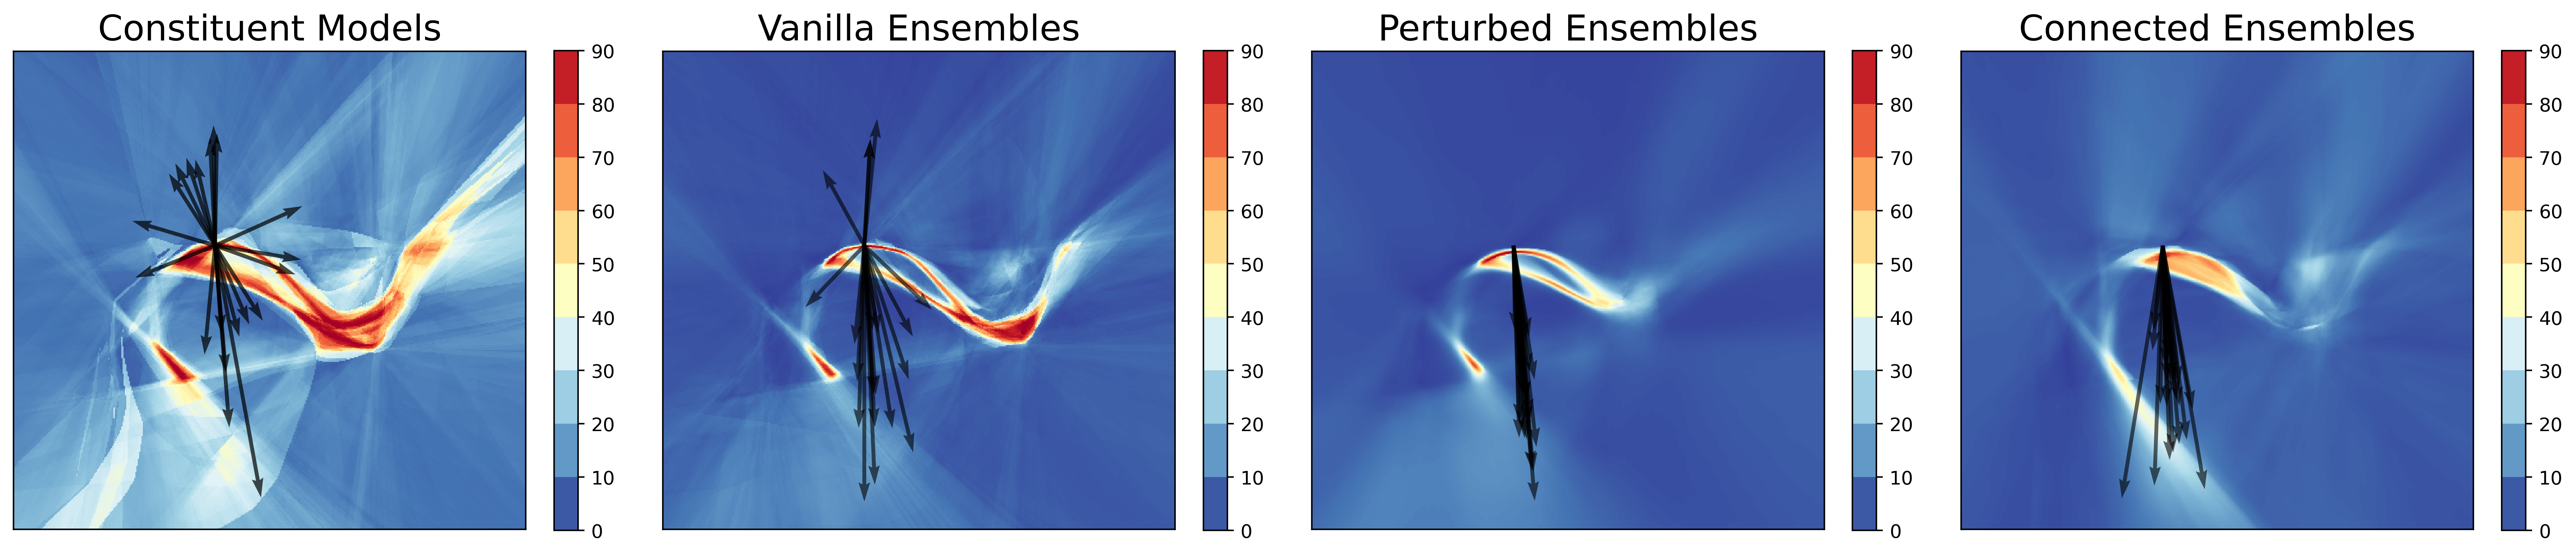
\includegraphics[width=\textwidth]{figures/toy_methods.png}
    \caption{\small Heatmaps of explanation disagreement (average pairwise angular difference between model gradients) for the described ensembling techniques, each constructed from four constituent models sampled from the underspecification set. \textbf{Left:} Baseline disagreements between equally performing models. Observe the high degree of dissimilarity between gradients (dark arrows) for a given test point. \textbf{Left Center to Right:} the efficacy of vanilla ensembles, ensembles via weight perturbation, and ensembles via mode connectivity on aligning explanations. For the same number of pre-trained models, local perturbations or global connections demonstrate potential for superior alignment of gradients between ensembles.}
    \label{fig:toy_methods}
\end{figure}

The process of averaging the outputs of local weight perturbations can be viewed as a mapping from the underspecification set of original models, to a reduced set of perturbed models, characterized by lower gradient variance. This \textit{shrinking} process necessitates fewer perturbed models to reach convergence in explanation alignment. In contrast, mode connectivity provides a more extensive traversal of the underspecification set, charting a broad range of models along the path between two endpoints. 
The following experiments demonstrate the efficacy of both exploratory methods in real-world scenarios. Notably, we find that their relative performance often hinges upon the unique characteristics of the given dataset, the explanation technique, and the particular model class used.